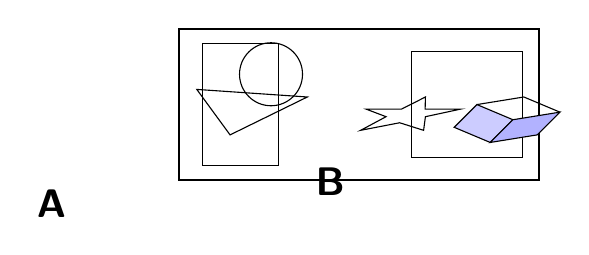
\begin{tikzpicture}[
    scale=0.5,
    font=\sffamily
]

% === Outer container A ===
\draw[thick] (-1,0,-1) rectangle (12,0,9);
\node[anchor=north west] at (-1,0,9) {\Large\textbf{A}};

% === Subregion A-left ===
\draw (0,0,0) rectangle (5,0,8);

% big triangle
\draw (1,0,3) -- (3,0,6) -- (4,0,3.5) -- cycle;

% circle
\draw (2.5,0,2) circle (0.8cm);

% === Subregion B ===
\draw (5.5,0,0.5) rectangle (11,0,7.5);
\node[anchor=north west] at (5.5,0,7.5) {\Large\textbf{B}};

% star
\draw (7,0,3.5)
    -- (7.3,0,4.3)
    -- (8.2,0,4.3)
    -- (7.5,0,4.8)
    -- (7.8,0,5.7)
    -- (7,0,5.2)
    -- (6.2,0,5.7)
    -- (6.5,0,4.8)
    -- (5.8,0,4.3)
    -- (6.7,0,4.3)
    -- cycle;

% cube (simplified)
\draw[fill=blue!20] (8.5,0,4) -- (9.8,0,5) -- (9.8,0,6.5) -- (8.5,0,5.5) -- cycle;
\draw[fill=blue!30] (9.8,0,5) -- (10.8,0,4.5) -- (10.8,0,6) -- (9.8,0,6.5) -- cycle;
\draw (8.5,0,4) -- (9.5,0,3.5) -- (10.8,0,4.5);

\end{tikzpicture}